\section{Evaluation Metrics}

The two main measurements for the performance of our new architecture are learning efficiency and transfer learning capability.
The learning efficiencies are measured in two different ways. First, the algorithm performance is compared with exisitng RL algorithms in terms of
convergence rate, which is measured in terms of number of episodes that the agent needs to get to an optimal policy.
Second, ILASP learning is measured in each episodes and time steps to see how the new algorithm refines its internal hypothesis over time.
Other common measurements in RL are XXX, XXX, but our primary goal of this research is data-efficient learning.

% We use GVG-AI Framework for our experiments, which was created for the General Video Gamea AI Competition\footnote{http://www.gvgai.net/},
% a game environment for an agent that should be able to play a wide variety of games without knowing which games are to be played.
\subsection{Experiment Platform}
We use the Video Game Definition Language (VGDL), which is a high-level description language for 2D video games providing a platform for computational intelligence research (\cite{Schaul2013}).
The VGDL allows users to easily craft their own environments, which makes us possible to do various experiments without relying on a default environment. The VGDL platform provides an interface with OpenAI Gym (\cite{Brockman2016}), which is a commonly used benchmark platform. 
The base game is a simple maze as shown in Figure \ref{VGDL_sample}.
There are 3 different types of cells: a goal cell, walls and paths. The agent can take 4 different actions: up, down, right and left.
The environment is not known to the agent in advance, and it attempts to find the goal by exploring the environment.

\begin{figure}[!ht!b]
    \centering
    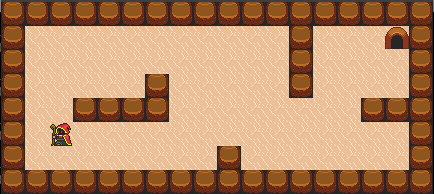
\includegraphics[width=0.5\textwidth]{./figures/experiment1}
    \caption{VGDL game example}
    \label{VGDL_sample}
    \end{figure}    
\subsection{Benchmark}
We use two existing reinforcement learning methods as benchmarks: Q-learning and tile-coding. 
Q-learning is most widely used technique for reinforcement learning. Given our environment is deterministic and discrete, this method works well in our environment.
Another benchmark is tile coding, which is a type of linear function approximation techniques described in Chapter XX.
The reason for using another extra benchmark is that the comparision with q-learning might not be a fair comparision,
since our algorithm has one extra assumptions: the agent knows surrounding information (whether there are walls in adjacent cells),
which is not a common assumption for Q-learning. Thus we incorporate the same surrounding information as features, and update the weights of each feature as a learning.
We compare the performance of our algorithm with these two methods.

\subsection{Parameters}
In all experiments, the agent receives -1 in any states except the goal state, where it gains a reward of 10.
Once the agent reaches the goal, or termination state, that episode is finished and the agent start the next episode from the starting point.
All the matrices that are used in the experiments are summarised in Table \ref{param}. 

\begin{table}[!ht!b]
\centering
\begin{tabular}{lll}
\hline
Parameter            & My algorithm    & Benchmark      \\ \hline
The number of episode& 100        & 100        \\
Time step per episode& 250        & 250        \\
The number of experiments& 30       & 30       \\
% Discount rate        & 0,5       & 1.4e-2       \\
Alpha                & N/A       & 0.5       \\
Epsilon              & 0.4        & 0.1        \\
\end{tabular}
\caption{Parameters of the initial and optimised fully connected network.}
\label{param}
\end{table}

Epsilon for our algorithm should be higher, since the agent follows the generated plan, 
whereas benchmark algorithms update value function with the degree of alpha. 
We conducted several experiments using different environments to highlight each aspect of the algorithm.

Since the performance of the agent is affected by the randomness of the exploration, 
and our algorithm is highly dependent on how quickly the agent finds the goal, 
each experiment is conducted 30 times and the perform is averaged across the experiments.
At each episode, we also measure the performance without exploration to see the pure optimal policy.

\section{Experiment Results}
\label{learning_evaluation}

\subsection{Experiment1}
The purpose of the first experiment is how the algorithm learns the model of the environment, or hypothesis in ILASP.
The environment are defined as a simple maze where the goal is located the right uppper corner as shown in Figure \ref{experiment1}.


The shortest path is XXX, so the maximum reward is XXX in this game. 

\begin{figure}[!htb]
\centering
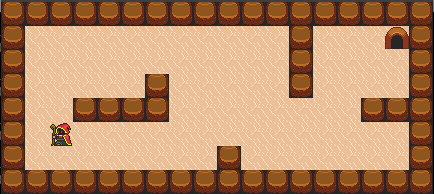
\includegraphics[width=0.5\textwidth]{./figures/experiment1}
\caption{Enviroment for experiment 1}
\label{experiment1}
\end{figure}

\begin{figure}[!htb]
\centering
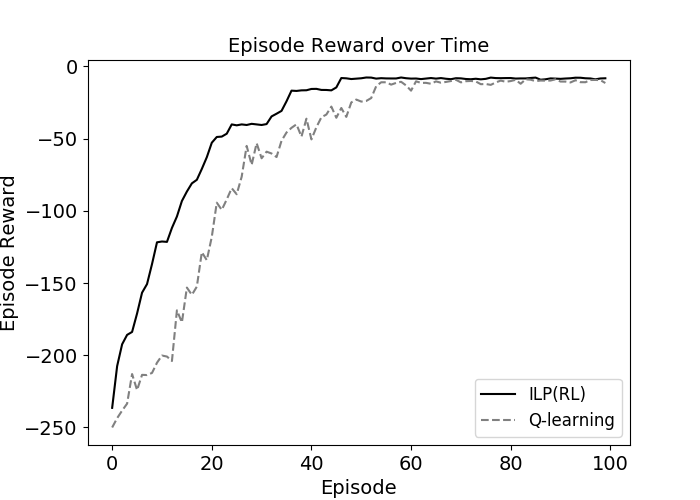
\includegraphics[width=1.0\textwidth]{./figures/experiment1_training}
\caption{Comparison of training performance between my algorithm and Q-learning}
\label{experiment1_training}
\end{figure}

Figure \ref{experiment1_training} shows the traning performance between our algorithm and Q-learning.
The convergence rate of our algorithm is faster than Q-learnig. This is because unlike Q-learning where the value function is updated with the rate of alpha, 
ILASP gradually build the model of the environment and use the background knowledge to accurately plan. 
The same trend is also shown in Figure \ref{experiment1_test}, where we measure only the performance of the policy without random exploration.

Overall this results shows that our algorithm converges to the optimal policy faster than transitional RL algorithm in a simple scenarios, achieving more data-efficient learning.

\begin{figure}[!htb]
\centering
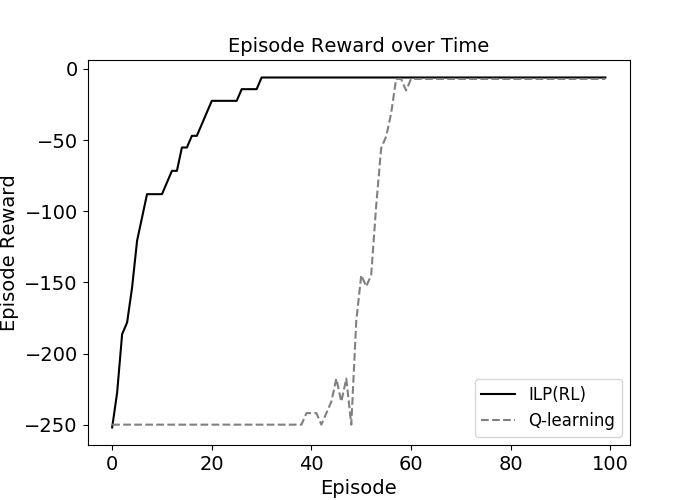
\includegraphics[width=1.0\textwidth]{./figures/experiment1_test}
\caption{Comparison of test performance between my algorithm and Q-learning}
\label{experiment1_test}
\end{figure}

\begin{figure}[!htb]
\centering
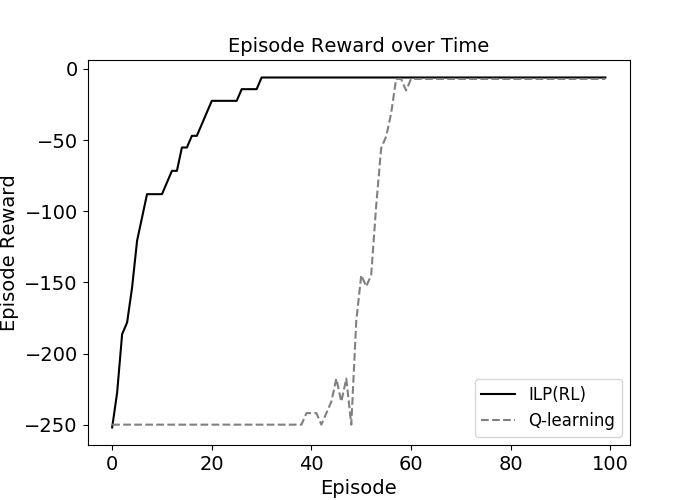
\includegraphics[width=1.0\textwidth]{./figures/experiment1_test}
\caption{PLACEHOLDER FOR ILASP}
\label{experiment1_test}
\end{figure}

The second improvement of our algorithm is transparency. 
Learnt hypotheses are shown in \ref{experiment1_hypothesis}, 
which is the rule of the game and easy to understand for human users. Since the learnt hypothesis is a general concept, which can be used in a different environmet. 
This transfer learning capability is also described in Experiement XX. 

ILASP learns the final hypothesis at time XX in episode 0.

\begin{equation}
\begin{split}
&\textsf{state\_after(V1) :- adjacent(right, V0, V1), state\_before(V1), action(right), wall(V0).}\\
&\textsf{state\_after(V0) :- adjacent(right, V0, V1), state\_before(V0), action(left), wall(V1).}\\
&\textsf{state\_after(V1) :- adjacent(down, V0, V1), state\_before(V1), action(down), wall(V0).}\\
&\textsf{state\_after(V1) :- adjacent(up, V0, V1), state\_before(V1), action(up), wall(V0).}\\
&\textsf{state\_after(V0) :- adjacent(right, V0, V1), state\_before(V1), action(right), not wall(V0).}\\
&\textsf{state\_after(V0) :- adjacent(left, V0, V1), state\_before(V1), action(left), not wall(V0).}\\
&\textsf{state\_after(V0) :- adjacent(down, V0, V1), state\_before(V1), action(down), not wall(V0).}\\
&\textsf{state\_after(V0) :- adjacent(up, V0, V1), state\_before(V1), action(up), not wall(V0).}
\end{split}
\end{equation}
\label{experiment1_hypothesis}

\subsection{Experiment2}

The first experiment might not be a fair comparision between our algorithm and Q-learning, since our algorithm has extra information about the surrounding information.
In order to have the same assumptions, we use function approximation for Q-learning.
Linear function approximation.

In this experiment, the performance of our algorithm remains the same as Experiment 1, but we use a different benchmark. 
% \begin{figure}[!htb]
% \centering
% 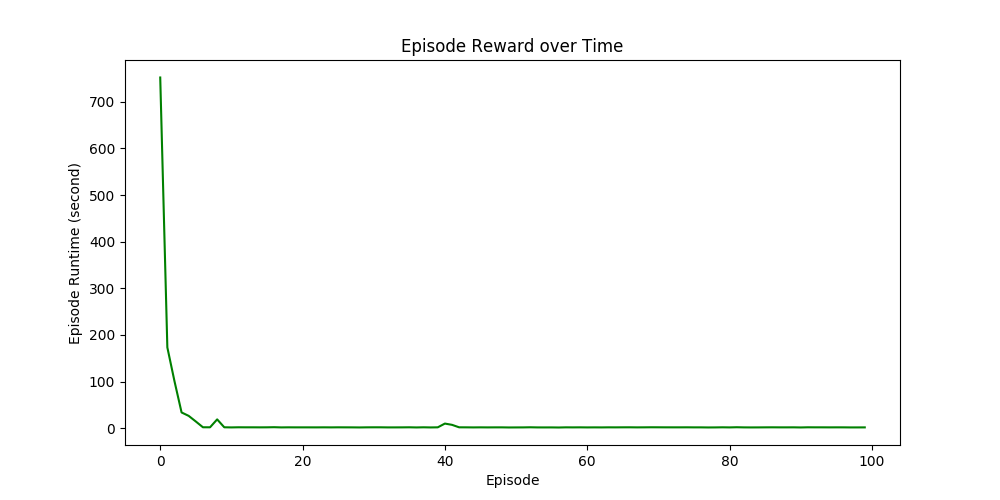
\includegraphics[width=1.0\textwidth]{./figures/placeholder}
% % 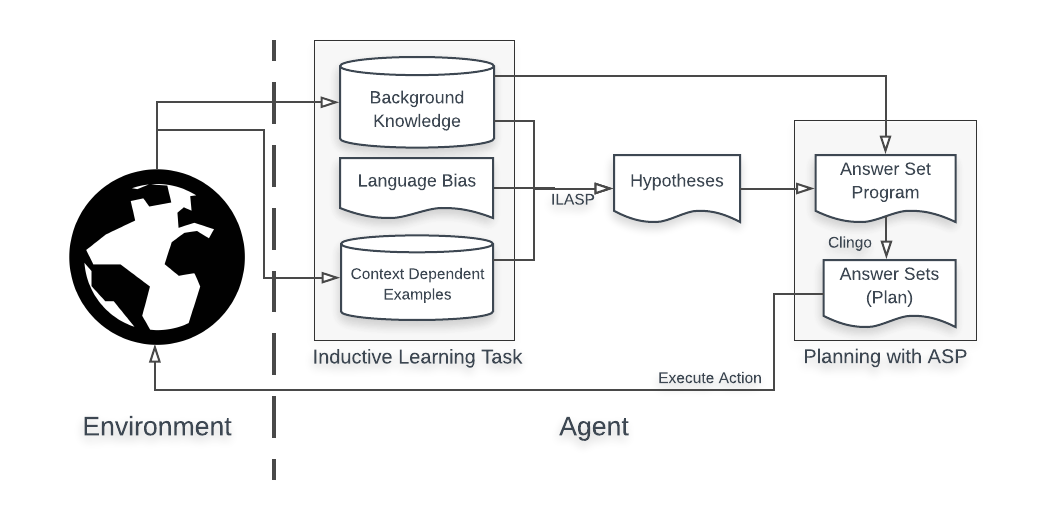
\includegraphics[width=10cm, height=9cm]{./figures/architecture}
% \caption{PLACEHOLDER}
% \label{proposed_architecture}
% \end{figure}
\newpage
\subsection{Experiment3}
% The game is designed such that

\begin{figure}[!htb]
\centering
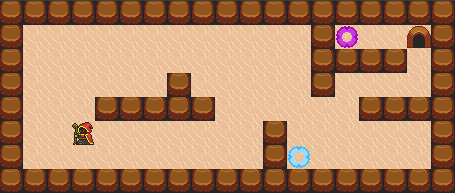
\includegraphics[width=0.5\textwidth]{./figures/experiment3}
\caption{Enviroment for experiment 3}
\label{experiment3}
\end{figure}

This experiment is conducted to see if the agent find a optimal path of using a teleport.
There are two ways to reach the goal: using a normal path or using a telport. 
The environment is designed such that using a teleport is a shorter path and therefore gives higher total reward. 

Compared to the first experiment, additional search space and concept are supplied as follow:
\begin{equation*}
\begin{split}
&\textsf{\#modeb(1, link\_start(var(cell)), (positive)).}\\
&\textsf{\#modeb(1, link\_dest(var(cell)), (positive)).}
\end{split}
\end{equation*}

Where an one way teleport link is added to the environment: link\_start takes the agent to link\_dest, but link\_dest does not take the agent back to link\_start.
The allows ILASP to learn additional hypothesis.
The full learning task for this experiment is in Appendix XX.

Once the agent steps onto a state where link\_start is located, it gets two positive experiences. 
In this game environment, the agent moves two cells in one time step instead of one cell per time step.


Also link\_start and link\_dest need to be stored in background knowledge rather than contex, 
because ILASP needs to learn different hypothesis for link and non-link case. 
link locations need to be available for all positive examples so that ILASP correctly learn non-link, which is shown in Figure XX below.


\begin{figure}[!htb]
\centering
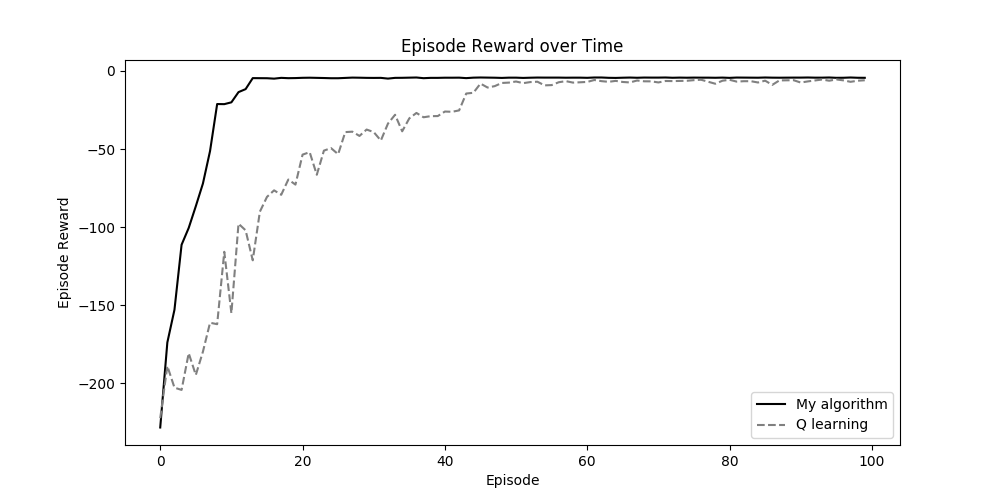
\includegraphics[width=1.0\textwidth]{./figures/experiment3_training}
\caption{Comparison of training performance between my algorithm and Q-learning}
\label{experiment3_training}
\end{figure}

The training performance shown in XX, which converges faster than XX. 

\begin{figure}[!htb]
\centering
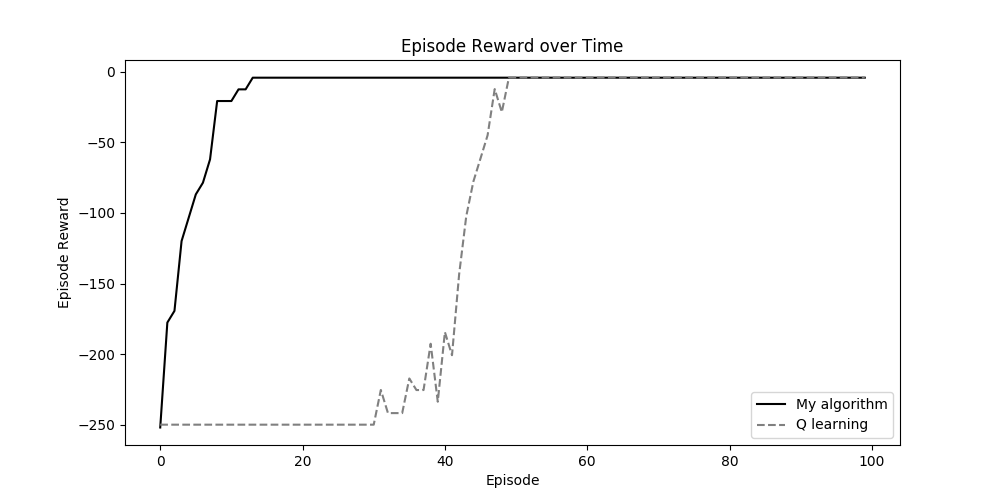
\includegraphics[width=1.0\textwidth]{./figures/experiment3_test}
\caption{Comparison of test performance between my algorithm and Q-learning}
\label{experiment3_test}
\end{figure}

\begin{figure}[!htb]
\centering
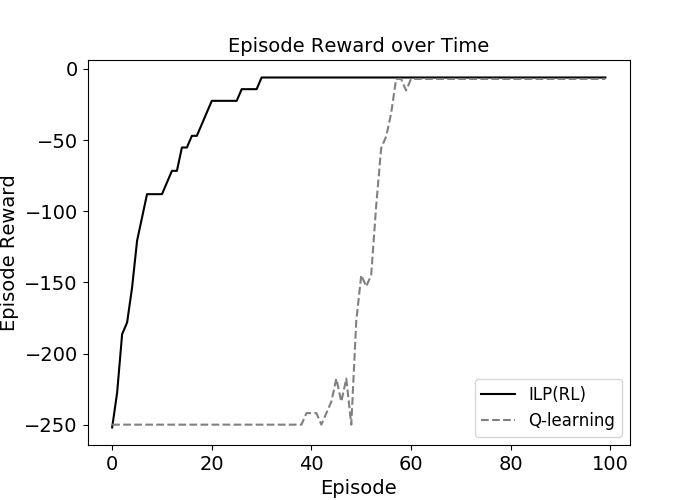
\includegraphics[width=1.0\textwidth]{./figures/experiment1_test}
\caption{PLACEHOLDER FOR ILASP}
\label{experiment1_test}
\end{figure}

ILASP learns the final hypothesis at time XX in episode 0.
To highlight the learning the new concept of teleport link, Figure XX is an intermediate incomplete hypothesis learnt by ILASP.
\begin{equation*}
\begin{split}
&\textsf{state\_after(V1) :- link\_dest(V1).}\\
&\textsf{state\_after(V0) :- link\_dest(V0), state\_before(V0), action(right).}\\
&\textsf{state\_after(V1) :- adjacent(left, V0, V1), state\_before(V0), action(right), not wall(V1).}\\
&\textsf{state\_after(V0) :- adjacent(left, V0, V1), state\_before(V1), action(left), not wall(V0).}\\
&\textsf{state\_after(V1) :- adjacent(up, V0, V1), state\_before(V0), action(down), not wall(V1).}\\
&\textsf{state\_after(V0) :- adjacent(up, V0, V1), state\_before(V1), action(up), not wall(V0).}\\
&\textsf{state\_after(V1) :- adjacent(left, V0, V1), state\_before(V1), action(left), wall(V0).}\\
&\textsf{state\_after(V1) :- adjacent(down, V0, V1), state\_before(V1), action(down), wall(V0).}\\
&\textsf{state\_after(V1) :- adjacent(up, V0, V1), state\_before(V1), action(up), wall(V0).}
\end{split}
\end{equation*}
These hypotheses are generated just after the agent steps onto the link. However, the first hypothesis says
whenever link\_dest is available state\_after is true. Since link\_dest is available in background knowledge rather than context, 
when solving for answer sets to generate a plan, it generates incorrect state\_after at every time step. 
However, as shown in Algorithms XX, these generated state\_after are all incorrect and therefore will be added to exclusions of the next positive examples. 
These exclusions will later refines hypotheses and results in Figure XX, the final complete hypotheses.

Learnt hypotheses are as follow:
\begin{equation*}
\begin{split}
&\textsf{state\_after(V1) :- link\_start(V0), link\_dest(V1), state\_before(V0).}\\
&\textsf{state\_after(V0) :- link\_dest(V0), state\_before(V0), action(right).}\\
&\textsf{state\_after(V1) :- adjacent(left, V0, V1), state\_before(V0), action(right), not wall(V1).}\\
&\textsf{state\_after(V0) :- adjacent(left, V0, V1), state\_before(V1), action(left), not wall(V0).}\\
&\textsf{state\_after(V1) :- adjacent(up, V0, V1), state\_before(V0), action(down), not wall(V1).}\\
&\textsf{state\_after(V0) :- adjacent(up, V0, V1), state\_before(V1), action(up), not wall(V0).}\\
&\textsf{state\_after(V1) :- adjacent(left, V0, V1), state\_before(V1), action(left), wall(V0).}\\
&\textsf{state\_after(V1) :- adjacent(down, V0, V1), state\_before(V1), action(down), wall(V0).}\\
&\textsf{state\_after(V1) :- adjacent(up, V0, V1), state\_before(V1), action(up), wall(V0).}
\end{split}
\end{equation*}

Compared the Experiment 1, there are two new hypotheses due to the presence of the teleport links. 
These learnt hypotheses are also applicables to an environment where there is not link, such as a game in experiment 1.
In this case, the first two hypotheses in Figure XX are never be used since the body predicates are never be true. 

\newpage

\subsection{Experiment4}

\begin{figure}[!htb]
\centerline{
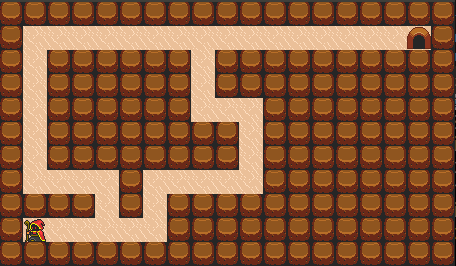
\includegraphics[width=0.5\textwidth]{./figures/experiment4_before}
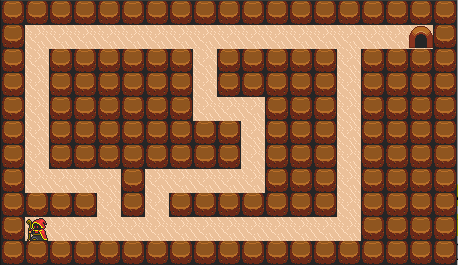
\includegraphics[width=0.5\textwidth]{./figures/experiment4_after}
}
\caption{Before (left) and after (right) transfer learning}
\label{experiment4}
\end{figure}

Finally, we investigated the potentials of transfer learning betweeen similar environments.
We trained the agent using the environment on the left in Figure XX, and transfer the learnt hypothesis as well as positive examples to a new environment.
Background knowledge are not transferred since they are different in a new environment. The agent starts with an empty background knowledge and gradually collects them
as it explore the environment. 
The goal position is the same as in the first game, but the routes to the goal are different.
While this is a limited transfer learning since the goal position is known in advance, this is still a useful transfer in cases where the rest of the environment changes,
such as XXX.

In this experiment, we compare the two learning performance: one with transfer learning and one without it. 
The result is shown in Figure XX.

Since the complete hypothesis is already known to the agent, it only needs to do planning. 

\begin{figure}[!htb]
\centering
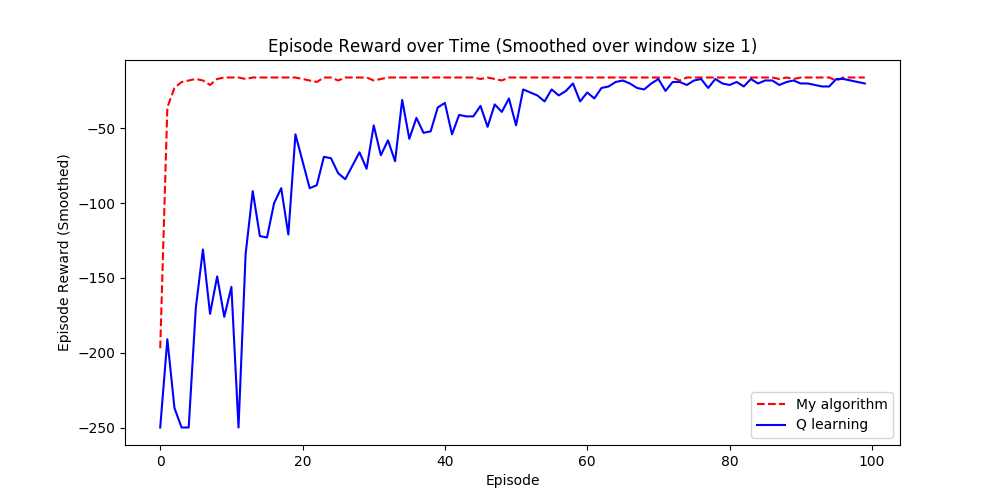
\includegraphics[width=1.0\textwidth]{./figures/experiment4_before_training}
\caption{Comparison of training performance between my algorithm and Q-learning (before transfer)}
\label{experiment3_training}
\end{figure}

\begin{figure}[!htb]
\centering
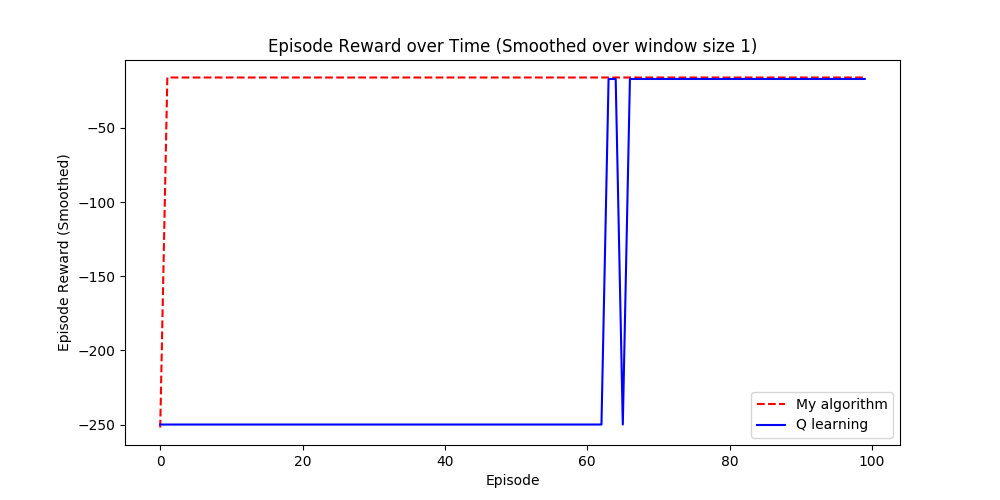
\includegraphics[width=1.0\textwidth]{./figures/experiment4_before_test}
\caption{Comparison of test performance between my algorithm and Q-learning (before transfer)}
\label{experiment3_test}
\end{figure}

\begin{figure}[!htb]
\centering
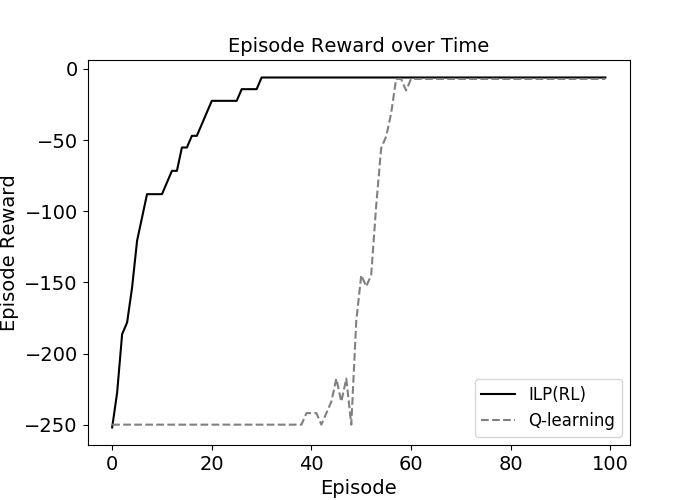
\includegraphics[width=1.0\textwidth]{./figures/experiment1_test}
\caption{PLACEHOLDER FOR ILASP}
\label{experiment1_test}
\end{figure}

These are the hypotheses we are transferring to a new environment.
\begin{equation*}
\begin{split}
 &\textsf{state\_after(V0) :- adjacent(right, V0, V1), state\_before(V1), action(right), not wall(V0).}\\
 &\textsf{state\_after(V0) :- adjacent(left, V0, V1), state\_before(V1), action(left), not wall(V0).}\\
 &\textsf{state\_after(V1) :- adjacent(down, V0, V1), state\_before(V0), action(up), not wall(V1).}\\
 &\textsf{state\_after(V0) :- adjacent(down, V0, V1), state\_before(V1), action(down), not wall(V0).}\\
 &\textsf{state\_after(V1) :- adjacent(right, V0, V1), state\_before(V1), action(right), wall(V0).}\\
 &\textsf{state\_after(V1) :- adjacent(left, V0, V1), state\_before(V1), action(left), wall(V0).}\\
 &\textsf{state\_after(V0) :- adjacent(up, V0, V1), state\_before(V0), action(down), wall(V1).}\\
 &\textsf{state\_after(V1) :- adjacent(up, V0, V1), state\_before(V1), action(up), wall(V0).}
\end{split}
\end{equation*}

\subsubsection{Transfer learning}

\begin{figure}[!htb]
\centering
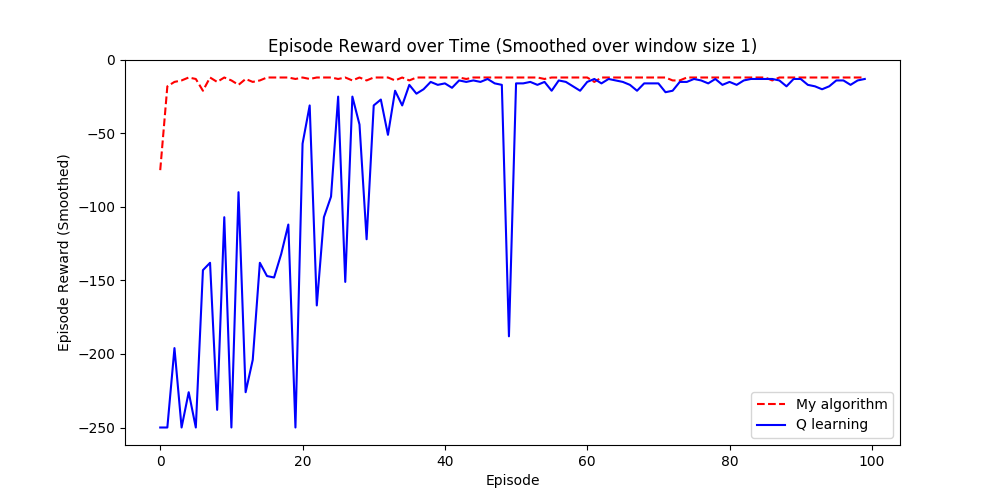
\includegraphics[width=1.0\textwidth]{./figures/experiment4_after_training}
\caption{Comparison of training performance between my algorithm and Q-learning (after transfer)}
\label{experiment3_training}
\end{figure}

\begin{figure}[!htb]
\centering
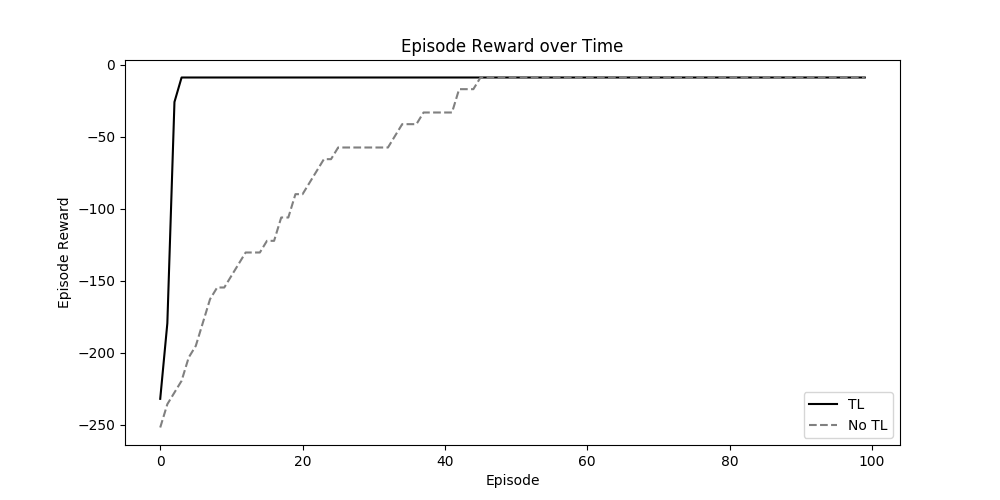
\includegraphics[width=1.0\textwidth]{./figures/experiment4_after_test}
\caption{Comparison of test performance between my algorithm and Q-learning (after transfer)}
\label{experiment3_test}
\end{figure}

These are the hypotheses we are transferring to a new environment.
\begin{equation*}
\begin{split}
\end{split}
\end{equation*}

\newpage
\subsection{Experiment5}
Finally the hypothesis is transferred to a new environment where there is a new concept that did not exist in the first environment
and therefore the agent needs to learn it after the hypothesis is transferred.
